\documentclass[a4paper, 12pt]{article}

\usepackage{graphicx}
\usepackage{subfigure}
\usepackage{enumitem}
\usepackage{adjustbox}
\usepackage{hyperref}
\usepackage{xepersian}
\settextfont{XB Niloofar.ttf}

\begin{document}

\title{نوروز در حرکت؛\\ تحلیل تردد جاده‌ای و گردشگری در ایران}
\author{گروه کفش مردانهٔ ورزشی}
\date{فروردین ۱۴۰۴}
\maketitle

\section{در جاده توسعه، پشت ترافیک مانده‌ایم...}
در حالی که در گزارش سال ۱۳۴۵، زمان متوسط سفر اصفهان-تهران ۳ روز با کالسکه ذکر شده بود، امروزه همان مسیر با خودروهای مدرن به ۵ ساعت کاهش یافته است؛ اما داده‌های ترددشمارها نشان می‌دهد که حجم تردد نوروزی به حدی زیاد است که میانگین سرعت در روزهای ابتدایی فروردین ۱۴۰۳ در برخی محورهای منتهی به اصفهان، تنها ۶۳ کیلومتر بر ساعت بوده است؛ گویی چرخ‌های توسعه آن‌قدرها هم سریع‌تر از اسب‌های قجری نمی‌دوند!

\begin{figure}[htbp]
    \centering
    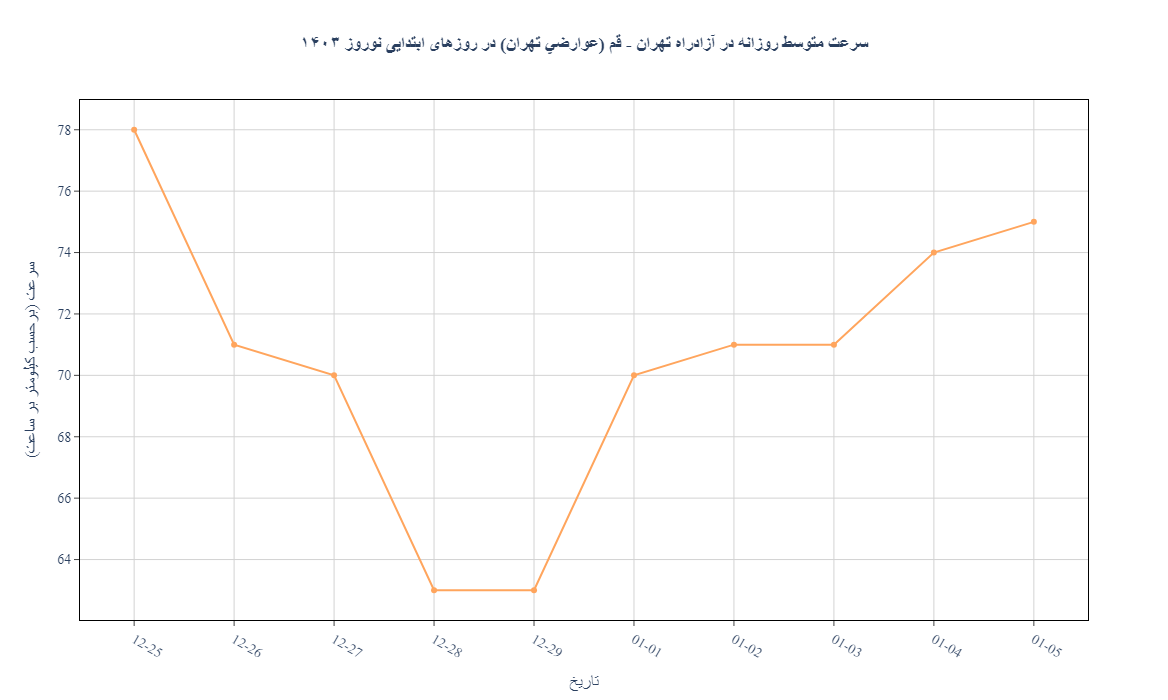
\includegraphics[width=1\textwidth]{first_part.png}
    \caption{سرعت متوسط سواری‌ها در آزادراه تهران-قم در روزهای ابتدایی نوروز ۱۴۰۳}
\end{figure}

اما این تعداد خودرو که موجب چنین ترافیکی شده‌اند، به کدام شهرها می‌روند؟ داده‌های ترددشمارها چه شهری را مقصد اول مسافران نوروزی معرفی می‌کنند؟ و آیا این حجم از سفرها نشان می‌دهد مردم به دنبال مقاصد تازه هستند یا همچنان پایبند به قطب‌های سنتی شناخته‌شده‌اند؟

\section{جاده‌هایی که زیر بار مسافران خم شده‌اند}
در هر دو سال ۱۴۰۲ و ۱۴۰۳، ده محور پرتردد کشور در ایام نوروز تقریبا بدون تغییر باقی مانده‌اند. بررسی داده‌های خودروهای کلاس یک (سواری و وانت) ترددشمارها نشان می‌دهد که محورهای واقع در محدوده‌های تهران، کرج و قزوین بیشترین حجم تردد را به خود اختصاص داده‌اند که با توجه به تمرکز جمعیتی بالا، موقعیت جغرافیایی به‌عنوان گذرگاه ورودی و خروجی پایتخت، و نقش آن‌ها به‌عنوان شاه‌راه‌های ارتباطی کشور، طبیعی است.
\\
\\
لازم به ذکر است که برخی از ترددشمارهای ذکرشده در میان ۱۰ محور پرتردد، در واقع مربوط به یک مسیر ترافیکی واحد هستند و تنها در نقاط مختلف مسیر یا در جهت مخالف نصب شده‌اند. ازاین‌رو، با هدف به‌دست‌آوردن تصویری دقیق‌تر از پراکندگی سفرها، این ترددشمارهای نزدیک به هم حذف شده و نماینده‌ای از هر محور پرتردد در نظر گرفته شده است. در ادامه، ۱۰ محور از میان پرترددترین محورها بر اساس داده‌های پالایش‌شده ارائه می‌گردد:
\begin{figure}[htbp]
    \centering
    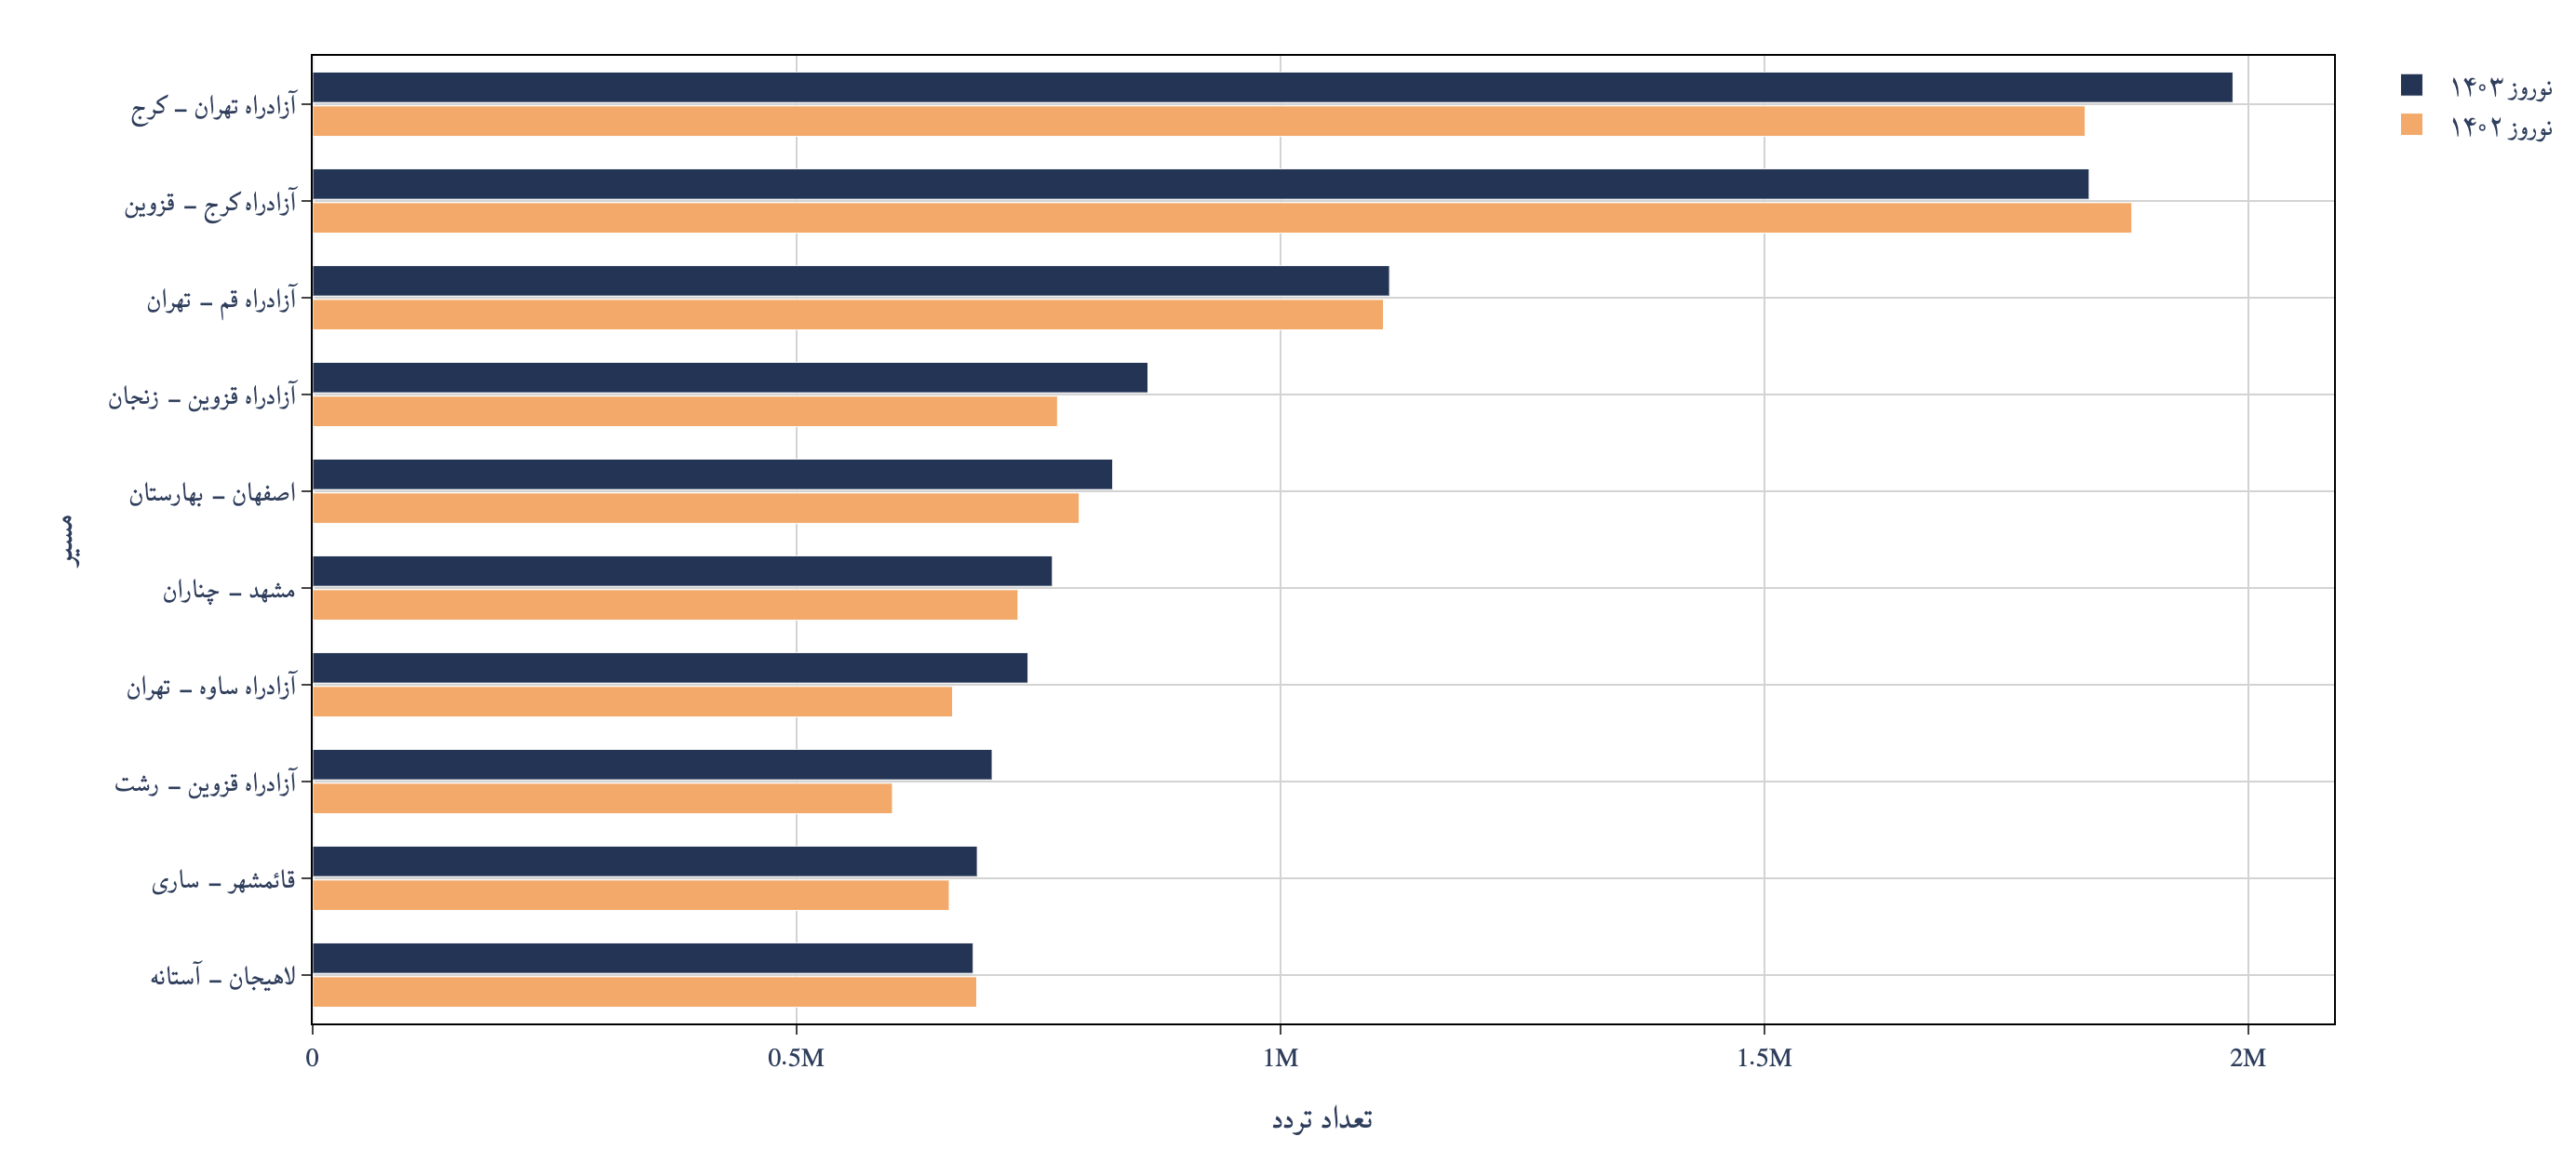
\includegraphics[width=1\textwidth]{most_taradod_roads.png}
    \caption{مقایسه میزان تردد خودروهای کلاس یک در محورهای پرتردد نوروز ۱۴۰۲ و ۱۴۰۳}
\end{figure}

\newpage
\section{از تردد تا سفر: یک سوء‌برداشت رایج}
بر اساس گزارش خبرگزاری صدا و سیما، معاون گردشگری سازمان میراث فرهنگی و گردشگری اعلام کرده است که سفرهای نوروزی در سال ۱۳۹۱ نسبت به سال قبل،
9.32
درصد رشد داشته است. با یک محاسبه‌ی آماری می‌توان دید که تعداد سفرهای نوروزی آن سال به حدود ۲۱۷ میلیون مورد رسیده؛ رقمی که تقریبا سه برابر جمعیت کشور در آن زمان بوده است!
\\

این در حالی‌ست که این آمار بر پایه داده‌های ترددشمارهای جاده‌ای -که صرفا تعداد عبور وسایل نقلیه از نقاط مشخصی در شبکه راه‌ها را ثبت می‌کنند- استخراج  گشته است؛ اما این داده‌ها محدودیت‌های روش‌شناختی خاص خود را دارند. از آن‌جا که یک خودرو ممکن است در جریان یک سفر از چندین ترددشمار عبور کند، در صورت جمع‌زدن ساده‌ی این داده‌ها، عدد حاصل می‌تواند به‌طور قابل توجهی بیشتر از واقعیت باشد. بنابراین، بدون درنظر گرفتن ماهیت این داده‌ها و تکراری بودن برخی از عبورها، آمار اعلام‌شده تصویری اغراق‌آمیز از میزان سفرهای نوروزی ارائه خواهد داد.
\\

از این‌رو، دستیابی به آماری دقیق‌تر از تعداد سفرها تنها از طریق ردیابی یکتای پلاک وسایل نقلیه ممکن خواهد بود؛ با این حال، تحلیل داده‌های ترددشمارها همچنان می‌تواند مبنای مناسبی برای مقایسه‌ی نسبی میان مسیرهای پررفت‌وآمد یا شهرهای مقصد گردشگری در نظر گرفته شود.


\section{به کدام مقاصد گردشگری باید بیشتر توجه کرد؟}
با آغاز هر نوروز، موج سفرهای جاده‌ای به‌سوی مقاصد گردشگری کشور شکل می‌گیرد و بررسی تغییرات این ترددها، می‌تواند تصویر روشنی از روند تقاضای سفر به ما بدهد. در این بخش، هدف ما مقایسه‌ی میزان تردد جاده‌ها در بازه‌ی نوروزی سال ۱۴۰۳ نسبت به سال ۱۴۰۲ است؛ مقایسه‌ای که می‌تواند به شناسایی مسیرهایی بینجامد که با رشد یا کاهش چشمگیر در حجم عبور و مرور مواجه بوده‌اند.
\\
محاسبه‌ی نرخ رشد تردد در مسیرهای مختلف به ما این امکان را می‌دهد که تغییر رفتار مسافران نوروزی را بهتر درک کنیم و همچنین مسیرهایی را شناسایی کنیم که به توجه مدیریتی بیشتری نیاز دارند؛ چه به‌دلیل افزایش فشار ترافیکی و نیاز به توسعه‌ی زیرساخت‌ها، و چه در نتیجه‌ی افت محسوس در تردد که ممکن است دلایل متنوعی از جمله تغییر در جذابیت مقصد، آب‌و‌هوا یا عوامل بیرونی دیگر، داشته باشد.
\\

با این حال، در حین بررسی داده‌ها، باید به محدودیت‌های آن نیز توجه کرد. بر اساس داده‌های ثبت‌شده توسط ترددشمارها در بازه‌ی ۲۹ اسفند تا ۱۳ فروردین، نرخ رشد تردد در برخی محورها از منفی ۹۶ درصد تا مثبت ۱۴۰۰ درصد متغیر بوده است! بازه‌ای بسیار گسترده که لزوماً بازتاب‌دهنده‌ی تغییرات واقعی سفرها نیست. چنین نوساناتی می‌تواند ناشی از نقص در داده‌ها، مسدود بودن برخی جاده‌ها در نوروز ۱۴۰۲ (مانند زمان بارش برف)، یا خطاهای اندازه‌گیری باشد.
\newpage
برای تحلیل دقیق‌تر نرخ رشد تردد در محورهای مختلف، نمودار جعبه‌ای نرخ رشد در بازه‌ی نوروزی (۲۹ اسفند تا ۱۳ فروردین) در دو سال ۱۴۰۲ و ۱۴۰۳ ترسیم شده است. با توجه به وجود داده‌های پرت قابل توجه ناشی از خطاهای اندازه‌گیری، بسته بودن مسیرها یا تغییرات در شبکه‌ی ترددشمارها، تصمیم گرفتیم تنها محورها با نرخ رشد در بازه‌ی کمی منطقی‌ترِ -۱۰۰٪ تا +۱۰۰٪ را در این تحلیل لحاظ کنیم.
\\
لازم به ذکر است از آن‌جا که در فاصله‌ی فروردین ۱۴۰۲ تا فروردین ۱۴۰۳ بیش از ۲۳۰ ترددشمار جدید در سطح کشور نصب شده‌اند، داده‌های مربوط به این دستگاه‌های تازه، از محاسبات نرخ رشد کنار گذاشته شده‌اند تا تحلیل نهایی از دقت بیشتری برخوردار باشد.

\begin{figure}[htbp]
    \centering
    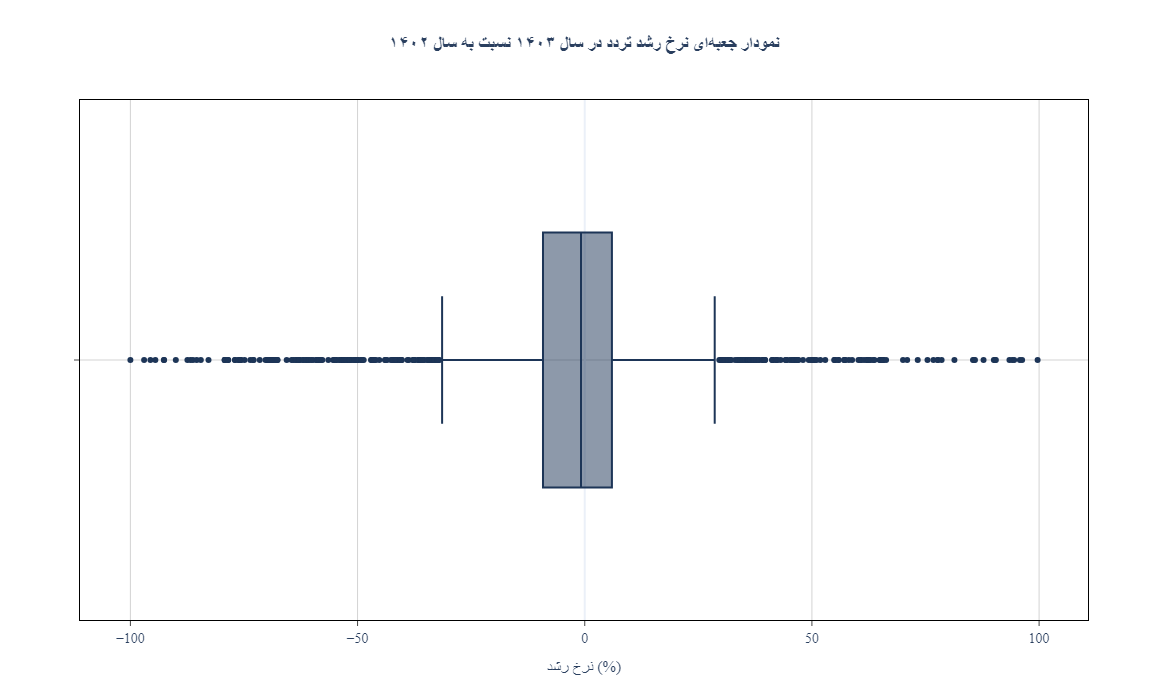
\includegraphics[width=1\textwidth]{growth.png}
    \caption{نمودار جعبه‌ای نرخ رشد تردد در سال ۱۴۰۳ نسبت به سال ۱۴۰۲}
\end{figure}


با بررسی نرخ رشد تردد در ۲۲۶۸ محور جاده‌ای کشور طی نوروز ۱۴۰۳ نسبت به مدت مشابه در سال ۱۴۰۲، میانه‌ی رشد تردد برابر با
82.0-
درصد و میانگین آن حدود
05.2-
درصد به‌دست آمده است. این دو شاخص آماری نزدیک به صفر نشان می‌دهند که در سطح کلان، تغییر محسوسی در میزان تردد جاده‌ای کشور رخ نداده و وضعیت سفرهای نوروزی در مجموع نسبتاً باثبات بوده است.

همچنین، یک چهارم پایین داده‌ها (25٪ پایین) رشد منفی بیش از
18.9
درصد داشته‌اند، در حالی‌که یک چهارم بالای داده‌ها افزایش بیش از
97.5
درصد
را تجربه کرده‌اند. این گستره‌ی نسبتاً متقارن، گواهی بر پراکندگی متعادل داده‌ها در اطراف صفر است.

در مجموع، این تحلیل نشان می‌دهد که الگوی کلی تردد جاده‌ای کشور در نوروز ۱۴۰۳ نسبت به سال پیش تغییر چشم‌گیری نداشته است، و افزایش یا کاهش‌های مشاهده‌شده در محورهای خاص، بیشتر بازتاب تفاوت‌های محلی یا مسائل فنی در ثبت داده‌ها هستند.

\subsection{مقایسه‌ی تردد روزانه در محورهای منتهی به شهر اصفهان}
برای تحلیل دقیق‌تر تغییرات ترافیکی در بازه‌ی نوروز، روند تردد روزانه در محورهای اصلی منتهی به شهر اصفهان در سال‌های ۱۴۰۲ و ۱۴۰۳ مورد بررسی قرار گرفته است. همان‌طور که در شکل زیر دیده می‌شود، این محورها که در زمره‌ی پرترددترین ورودی‌های شهر اصفهان در ایام تعطیلات به‌شمار می‌روند، به شرح زیر هستند:
\begin{figure}[htbp]
    \centering
    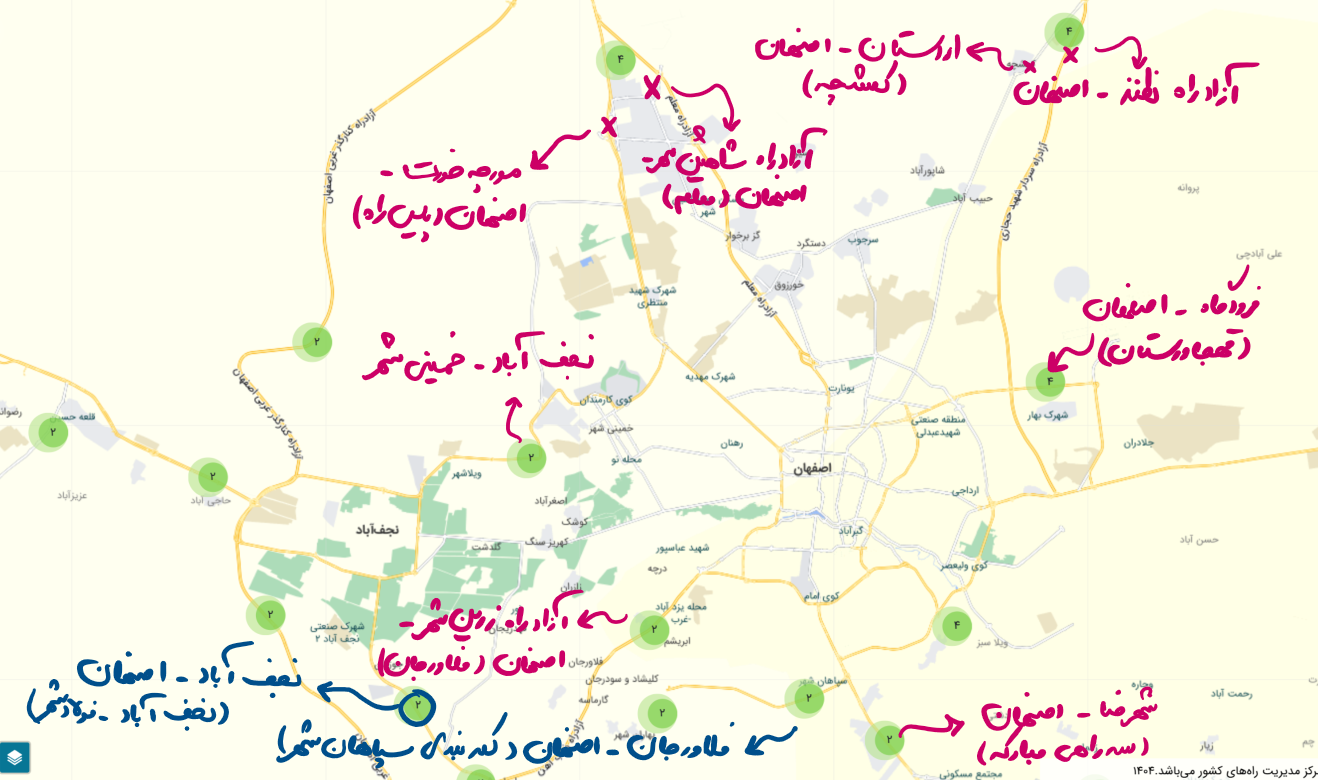
\includegraphics[width=1\textwidth]{isfahan_141.png}
    \caption{نقشه‌ی محورها و آزادراه‌های اصلی ورودی به اصفهان}
\end{figure}

% \begin{itemize}[itemsep=0.5pt]
%     \item آزادراه نطنز - اصفهان (نطنز)
%     \item آزادراه زرين شهر - اصفهان (فلاورجان)
%     \item آزادراه شاهين‌شهر - اصفهان (آزادراه معلم)
%     \item محور فرودگاه - اصفهان (قهجاورستان)
%     \item محور مورچه‌خورت - اصفهان (پليس‌راه)
%     \item محور شهرضا - اصفهان (سه‌راهی مبارکه)
%     \item محور اردستان - اصفهان (کمشچه)
%     \item محور نجف‌آباد - اصفهان (نجف‌آباد - فولادشهر)
%     \item محور فلاورجان - اصفهان (کمربندی سپاهان شهر)
% \end{itemize}

\newpage
بررسی داده‌های روزانه‌ی بازه‌ی ۲۹ اسفند تا ۱۳ فروردین، برای هر دو سال ۱۴۰۲ و ۱۴۰۳ نشان می‌دهد که در ۷ محور از میان این ۹ محور، نرخ رشد تردد منفی بوده است؛ به‌عنوان مثال، آزادراه نطنز-اصفهان با کاهش شدید ۵۳٪، بیشترین افت را داشته و پس از آن آزادراه زرین‌شهر–اصفهان با ۳۳٪ کاهش و آزادراه شاهین‌شهر-اصفهان با ۲۸٪ کاهش قرار دارند. نمودارهای خطی زیر، نشان‌دهنده‌ی حجم تردد روزانه در این دو سال و در محورهای ذکر شده می‌باشد:

\begin{figure}[htbp]
    \centering
    \subfigure[آزادراه نطنز-اصفهان]{
        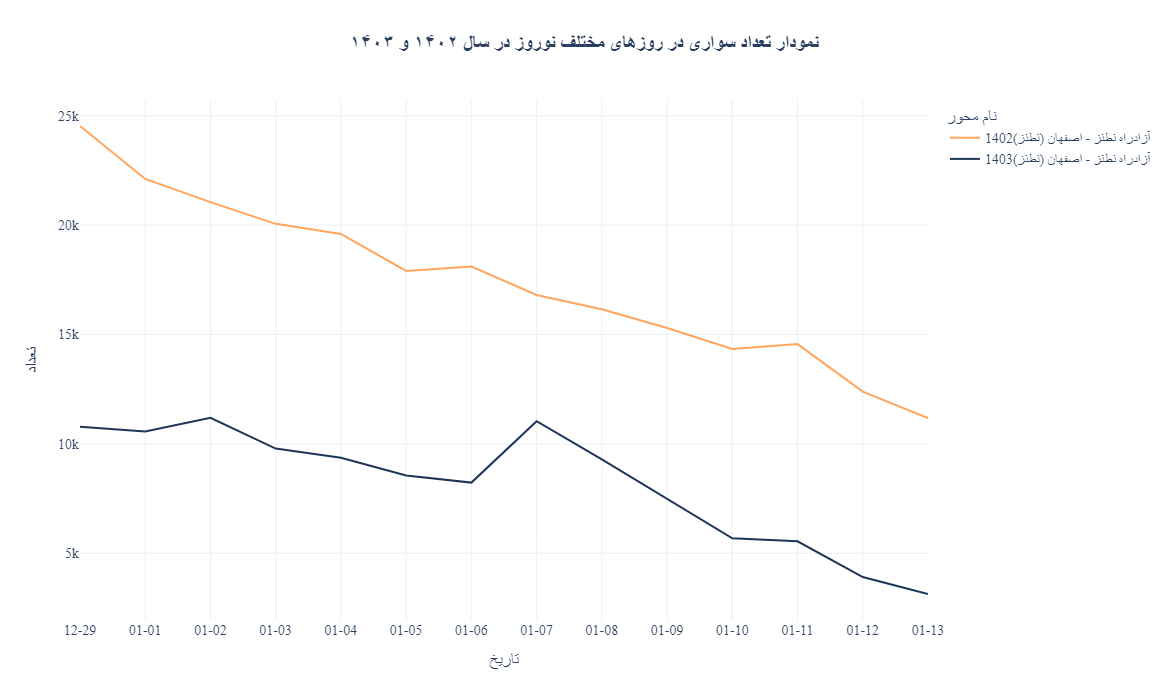
\includegraphics[width=0.8\textwidth]{compare_214902.png}
    }
    \subfigure[آزادراه زرین شهر-اصفهان]{
        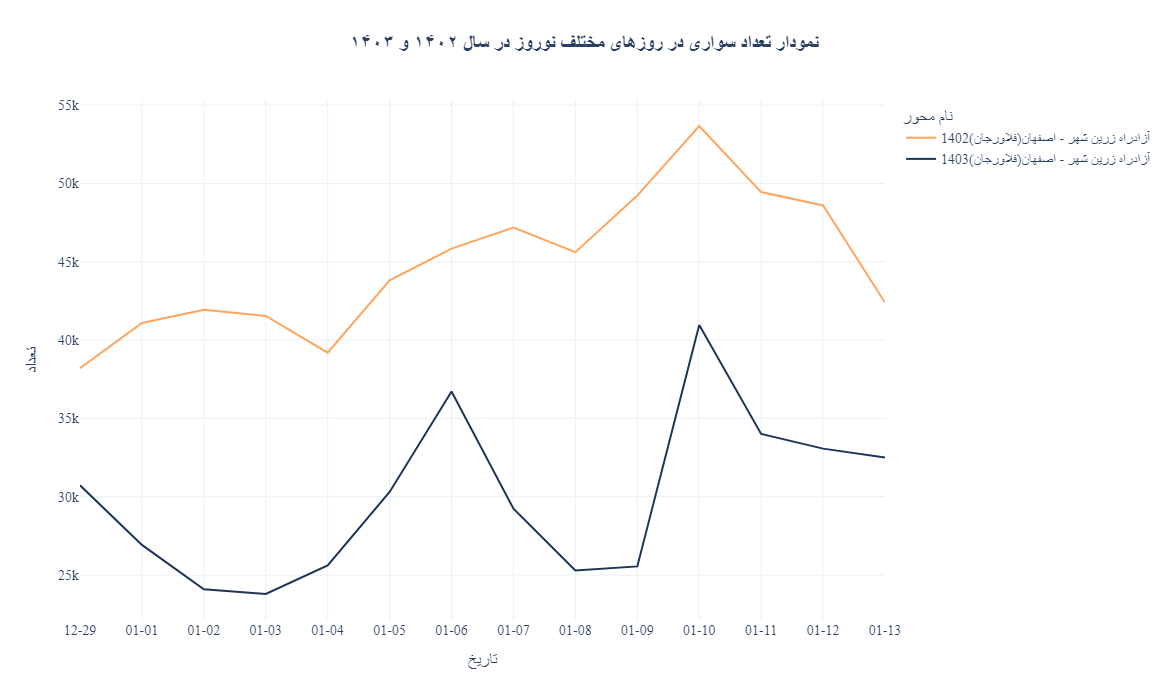
\includegraphics[width=0.8\textwidth]{compare_213163.png}
    }
    % \subfigure[آزادراه شاهین شهر-اصفهان]{
    %     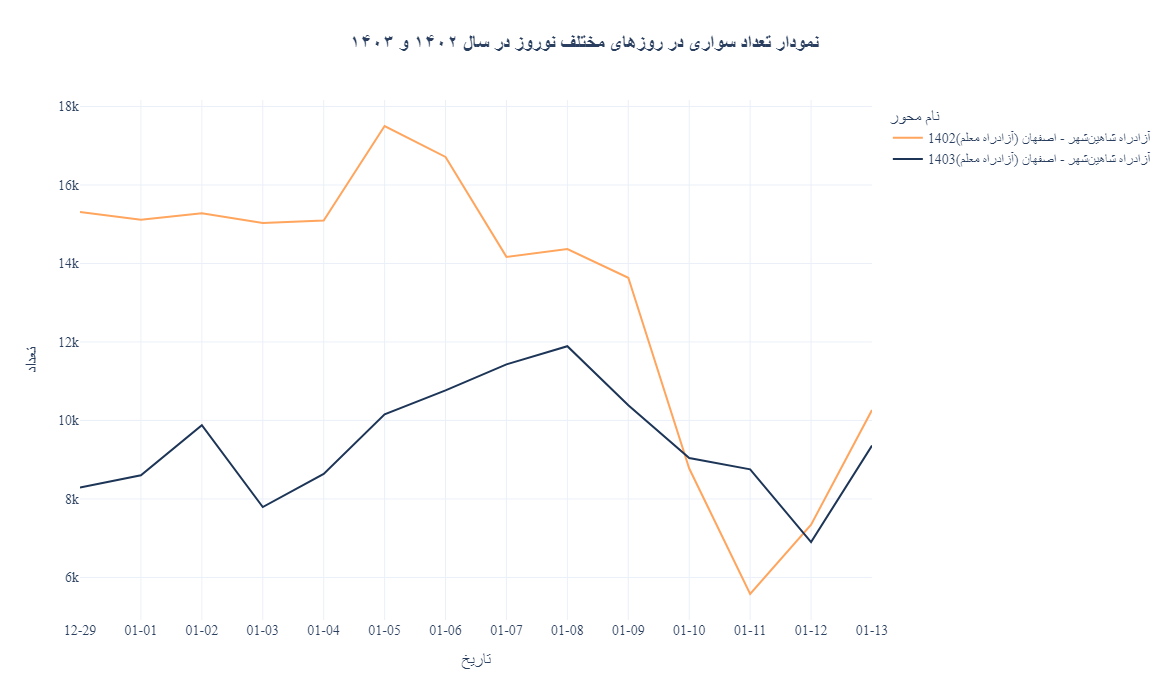
\includegraphics[width=1.1\textwidth]{compare_215104.png}
    % }
    % \subfigure[آزادراه فلاورجان-اصفهان]{
    %     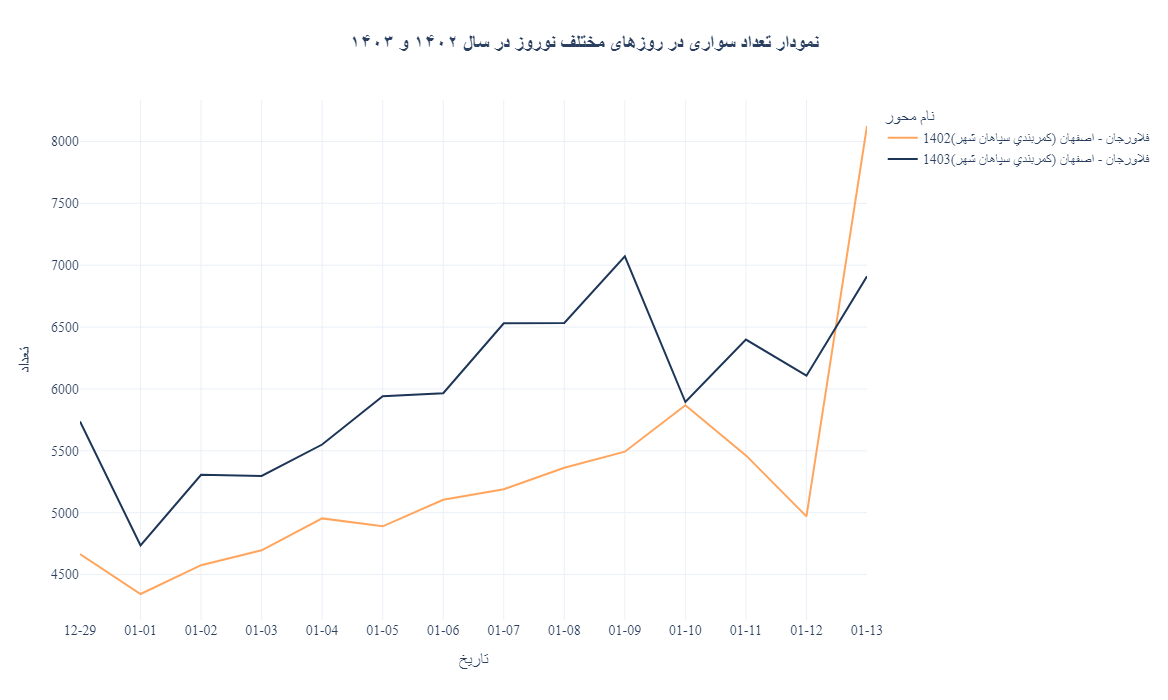
\includegraphics[width=1.1\textwidth]{compare_213279.png}
    % }
    % \subfigure[آزادراه نجف آباد-اصفهان]{
    %     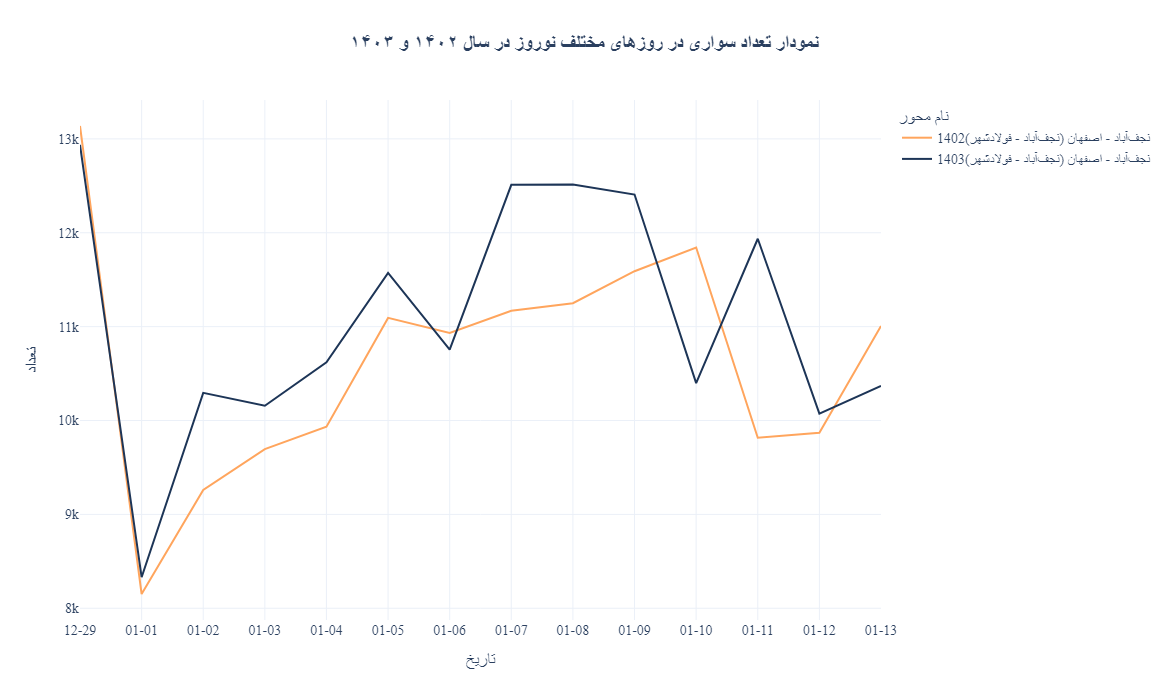
\includegraphics[width=1.1\textwidth]{compare_214762.png}
    % }
    \caption{نمودار تعداد سواری‌ها در آزادراه‌های مختلف منتهی به اصفهان در نوروز ۱۴۰۲ و ۱۴۰۳}
\end{figure}
\newpage
\begin{figure}[htbp]
    \centering
    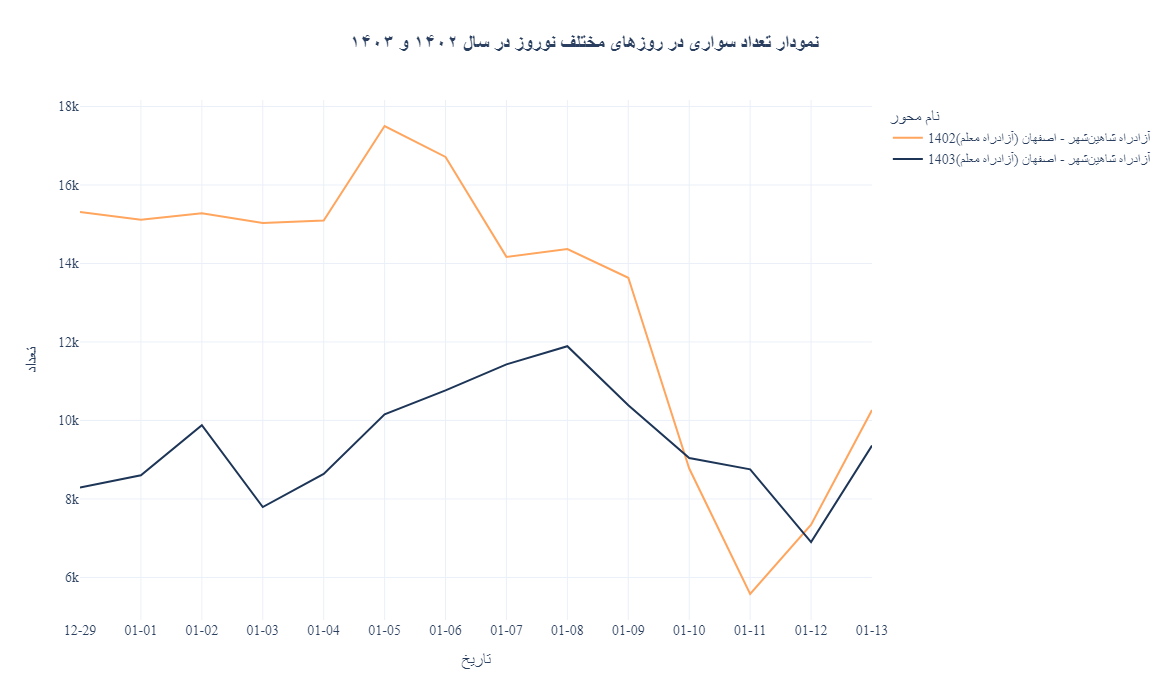
\includegraphics[width=0.8\textwidth]{compare_215104.png}
    \caption{نمودار تعداد سواری‌ها در آزادراه شاهین شهر-اصفهان در نوروز ۱۴۰۲ و ۱۴۰۳}
\end{figure}

از سوی دیگر، تنها ۲ محور فلاورجان–اصفهان و نجف‌آباد-اصفهان به ترتیب با ۱۳.۹٪ افزایش و  ۴.۱٪ افزایش، رشد مثبت داشته‌اند. نمودارهای خطی زیر، نشان‌دهنده‌ی حجم تردد روزانه در این دو سال و در محورهای ذکر شده می‌باشد:

\newpage 
\begin{figure}[htbp]
    \centering
    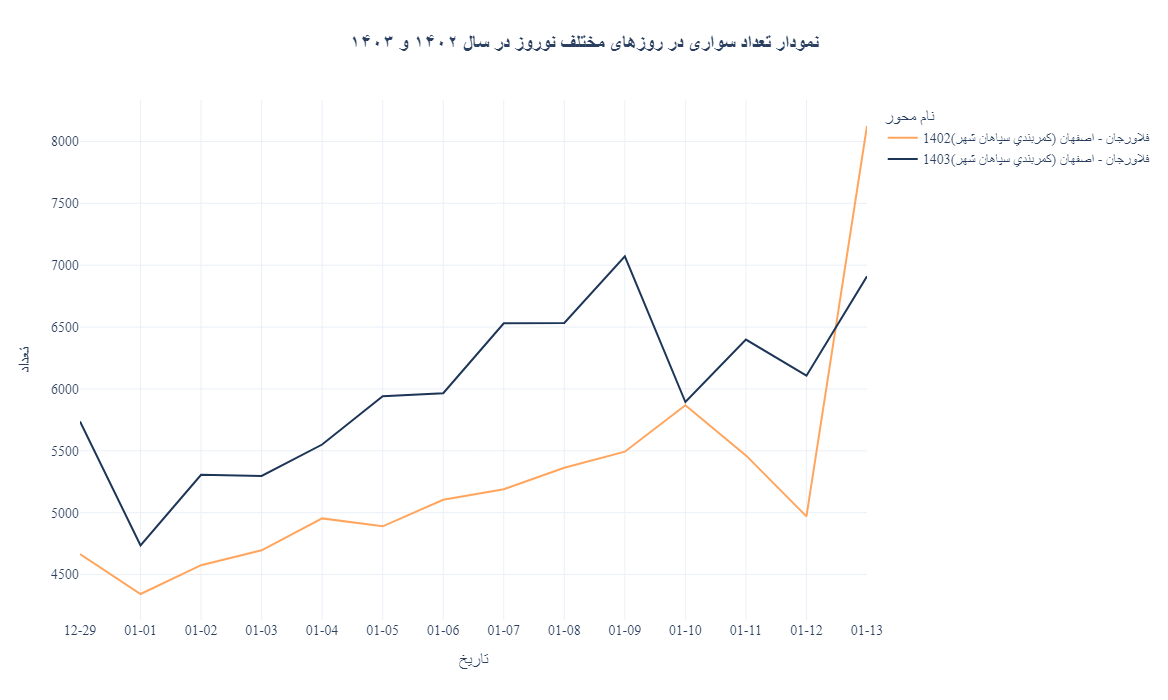
\includegraphics[width=1\textwidth]{compare_213279.png}
    \caption{نمودار تعداد سواری‌ها در آزادراه فلاورجان - اصفهان در نوروز ۱۴۰۲ و ۱۴۰۳}
\end{figure}
کلی چیز

\newpage
\section{پیک زمانی}
سفرهای نوروزی، برخلاف تصور رایج، تنها محدود به یکی دو روز ابتدایی تعطیلات نیستند؛ بلکه در بازه‌ی زمانی تقریبا دو هفته‌ای، چندین نقطه‌ی اوج در حجم ترددهای جاده‌ای دیده می‌شود. داده‌های ترددشمارها نشان می‌دهند که این پیک‌ها معمولاً با شروع تعطیلات رسمی، روزهای منتهی به تحویل سال و همچنین روزهای پایانی تعطیلات و بازگشت به شهرهای مبدا همزمان می‌شوند.

\begin{figure}[htbp]
    \centering
    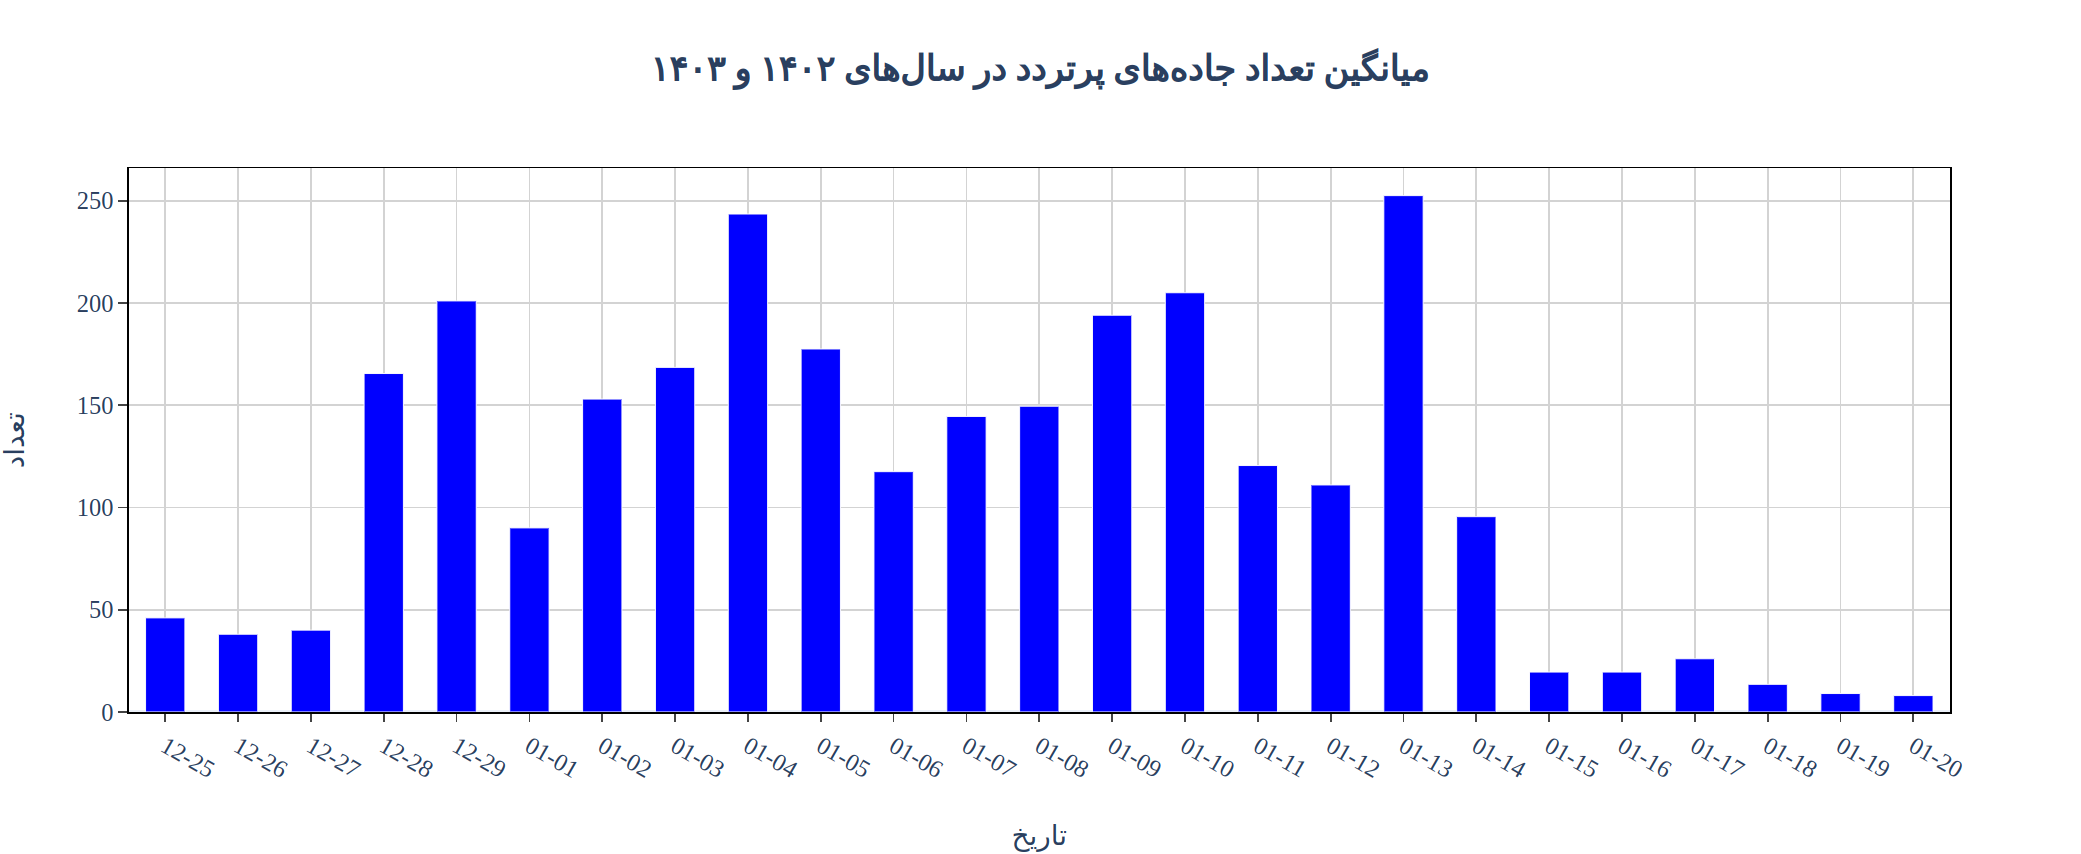
\includegraphics[width=0.8\textwidth]{peaks-pics/count_mean.png}
    \caption{نمودار تعداد سواری‌ها در آزادراه شاهین شهر-اصفهان در نوروز ۱۴۰۲ و ۱۴۰۳}
\end{figure}

بررسی روزانه‌ی تعداد جاده‌های پرتردد در بازه‌ی ۱۰ اسفند تا ۲۰ فروردین برای سال‌های ۱۴۰۲ و ۱۴۰۳ نشان‌دهنده‌ی الگوهای مشخصی در رفتار سفرهای نوروزی است. از تاریخ ۲۸ اسفند، تعداد جاده‌های پرتردد به‌صورت ناگهانی افزایش پیدا می‌کند. رشد تعداد جاده‌های پرتردد تا ۱۴ فروردین ادامه پیدا می‌کند که ناشی از سفرهای نوروزی‌ست.

\begin{figure}[htbp]
    \centering
    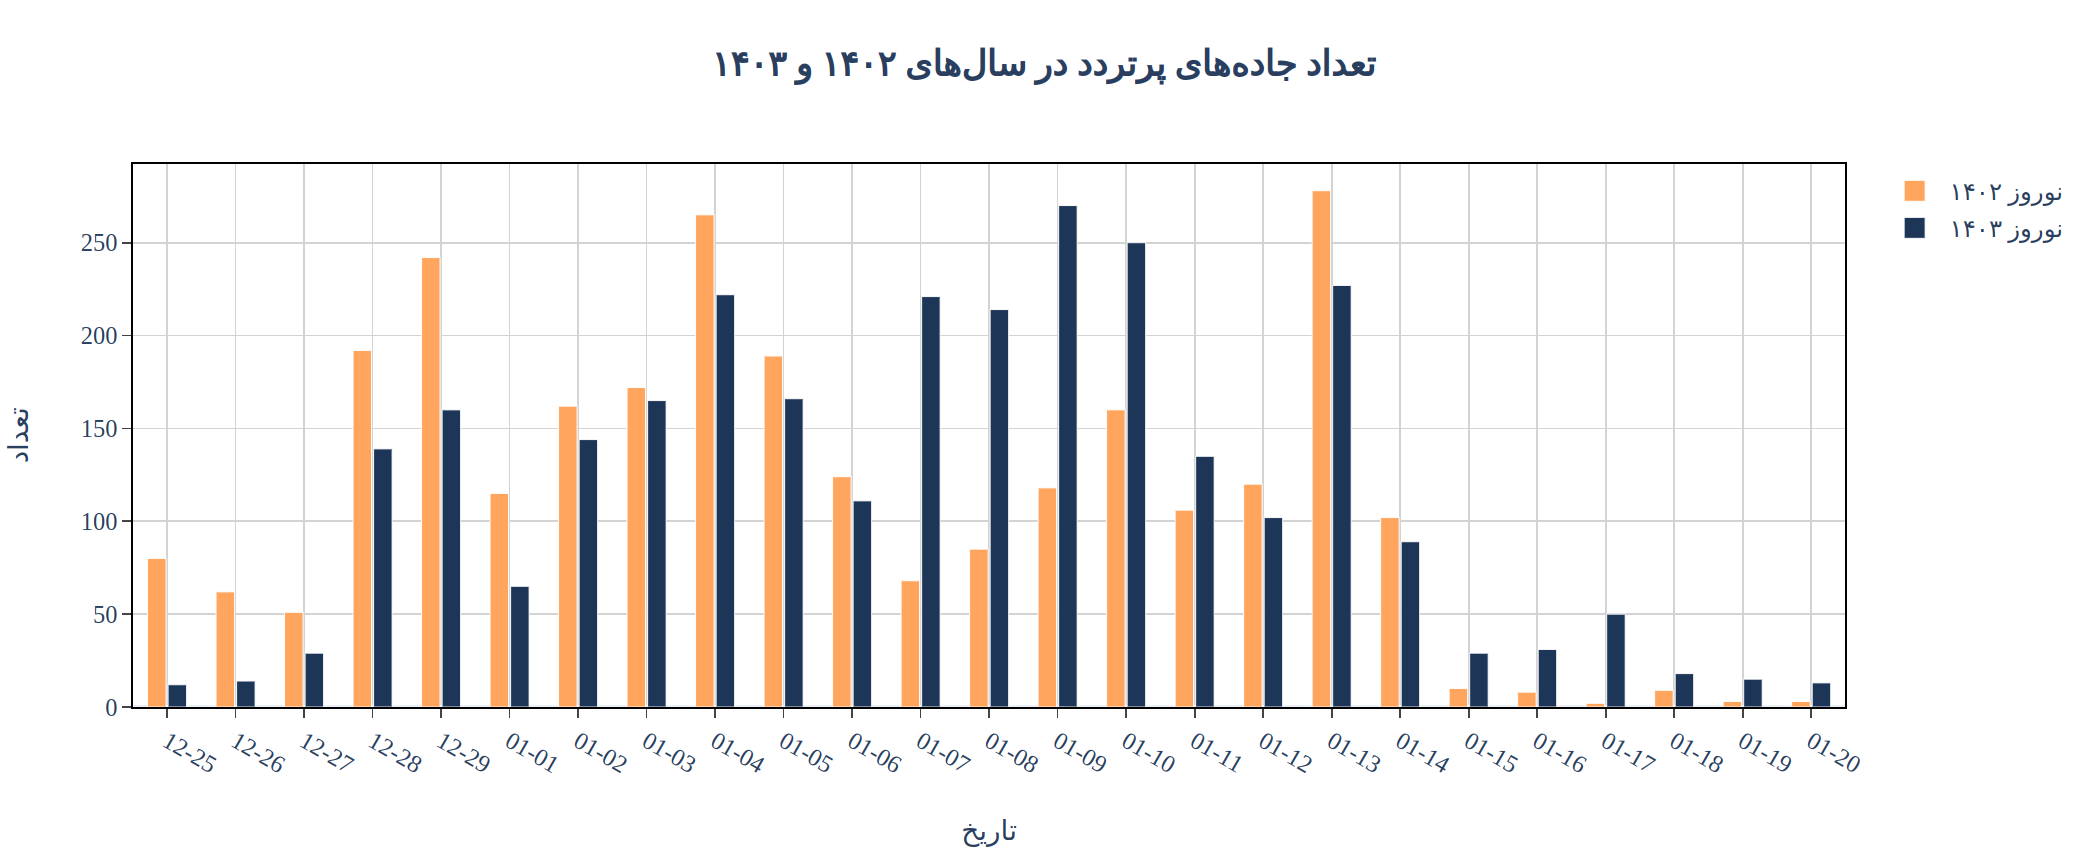
\includegraphics[width=0.8\textwidth]{peaks-pics/count_both.png}
    \caption{نمودار تعداد سواری‌ها در آزادراه شاهین شهر-اصفهان در نوروز ۱۴۰۲ و ۱۴۰۳}
\end{figure}

برای بررسی دقیق‌تر الگوی سفرها در تعطیلات نوروزی، بازه‌ی بین ۲۸ اسفند تا ۱۴ فروردین به‌عنوان دوره‌ی اوج سفرها مورد توجه قرار خواهد گرفت.
\medskip
 در سال ۱۴۰۲، بررسی داده‌ها نشان می‌دهد که روزهای ۲۹ اسفند، ۴ فروردین و ۱۳ فروردین پرترددترین روزها بوده‌اند؛ این روزها در دو سوی طیف تعطیلات قرار دارند و نماینده‌ی موج رفت و موج بازگشت سفرها هستند. در ادامه، روزهایی مانند ۲۸ اسفند، ۲ تا ۵ فروردین و ۱۰ فروردین نیز سطح قابل‌توجهی از تردد را به خود اختصاص داده‌اند، اما شدت تردد آن‌ها به اندازه‌ی سه روز ذکر شده نیست. در مقابل، روزهای ۷ و ۸ فروردین نسبت به سایر ایام نوروز، میزان تردد کمتری داشته‌اند و به‌نوعی بازه‌ی میانی و کم‌رفت‌وآمد تعطیلات به‌حساب می‌آیند.

یکی از نکات قابل‌توجه در سال ۱۴۰۲، قرار گرفتن ۲۹ اسفند ۱۴۰۱ در روز دوشنبه بود که با توجه به تعطیلی آن روز، بسیاری از افراد مرخصی خود را با این تعطیلی‌ها هم‌زمان کرده و زودتر سفرهای نوروزی‌شان را آغاز کرده‌اند. همین موضوع، ترافیک بالای این روز را تا حد زیادی توضیح می‌دهد.

\begin{figure}[htbp]
    \centering
    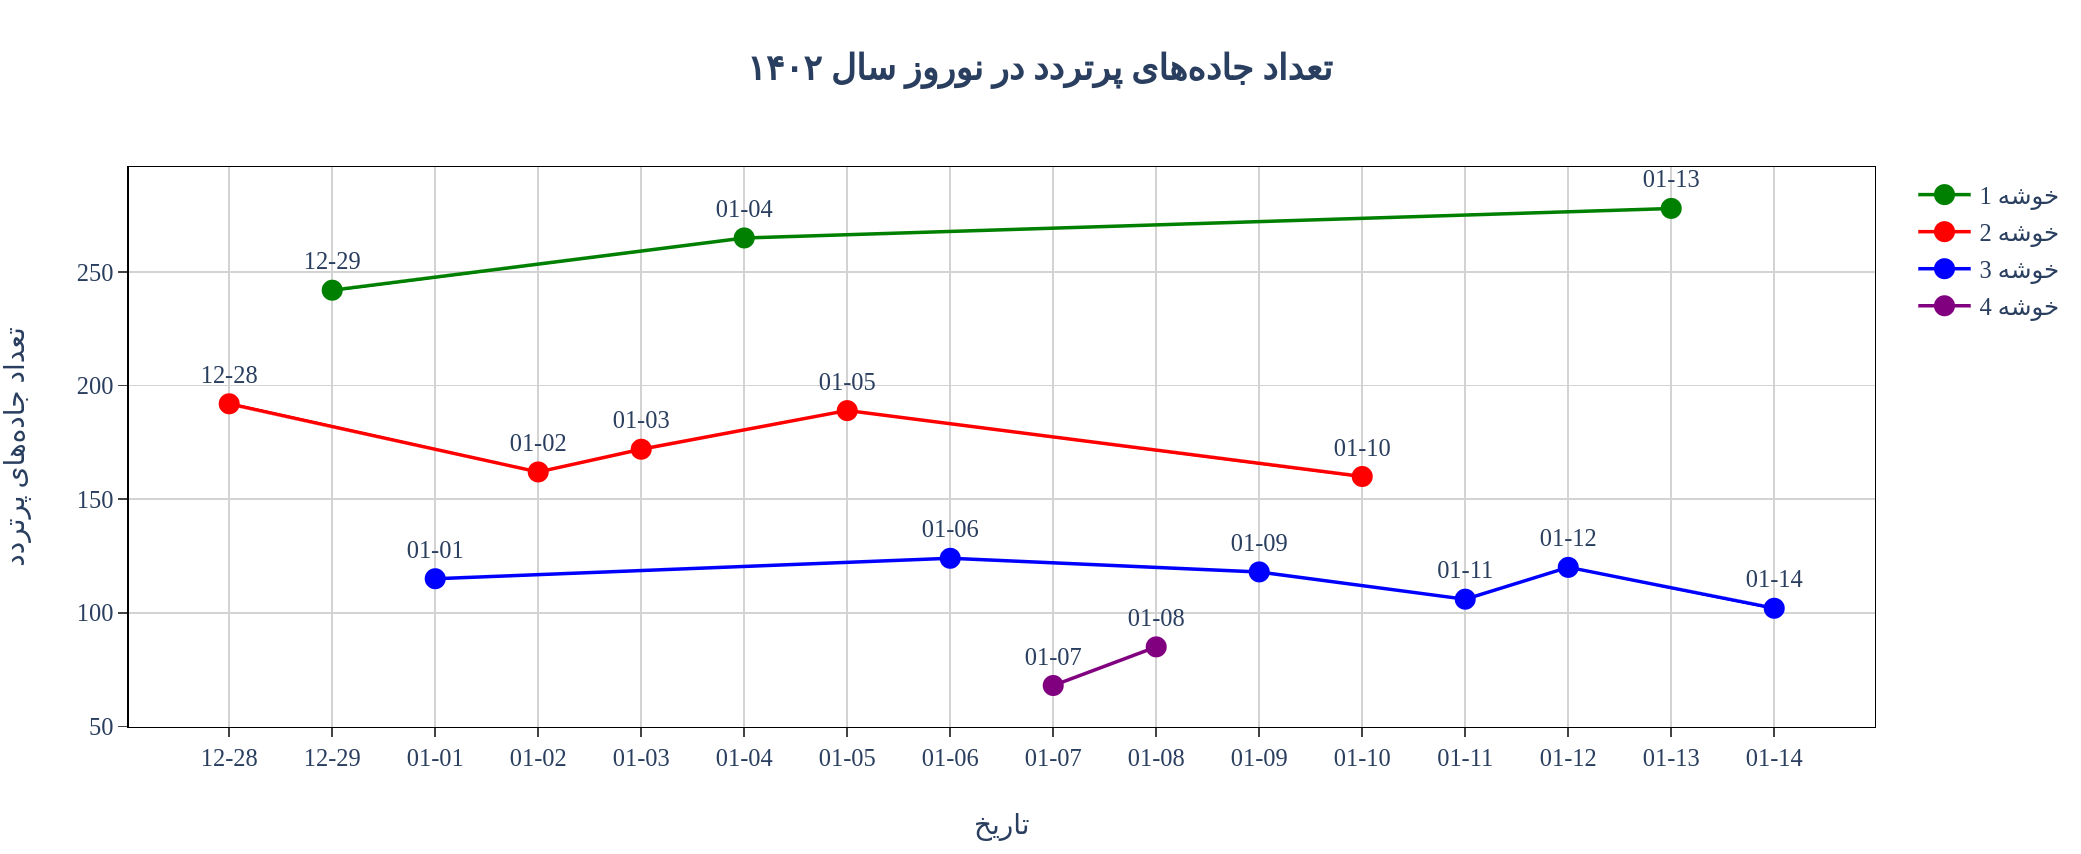
\includegraphics[width=0.8\textwidth]{peaks-pics/cluster1402.png}
    \caption{نمودار تعداد سواری‌ها در آزادراه شاهین شهر-اصفهان در نوروز ۱۴۰۲ و ۱۴۰۳}
\end{figure}

در سال ۱۴۰۳، پرترددترین روزها شامل ۴، ۷، ۸، ۹، ۱۰ و ۱۳ فروردین بوده‌اند. برخلاف الگوی سال قبل که از اواخر اسفند شدت می‌گرفت، در این سال موج اصلی سفرها با تاخیر آغاز شده و یک اوج در هفته اول و یک اوج در هفته دوم مشاهده می‌شود. لازم به ذکر است که تردد زیاد ۱۳ فروردین نیز به عنوان روز بازگشت مسافران در هر دو سال به خوبی دیده می‌شود.


\begin{figure}[htbp]
    \centering
    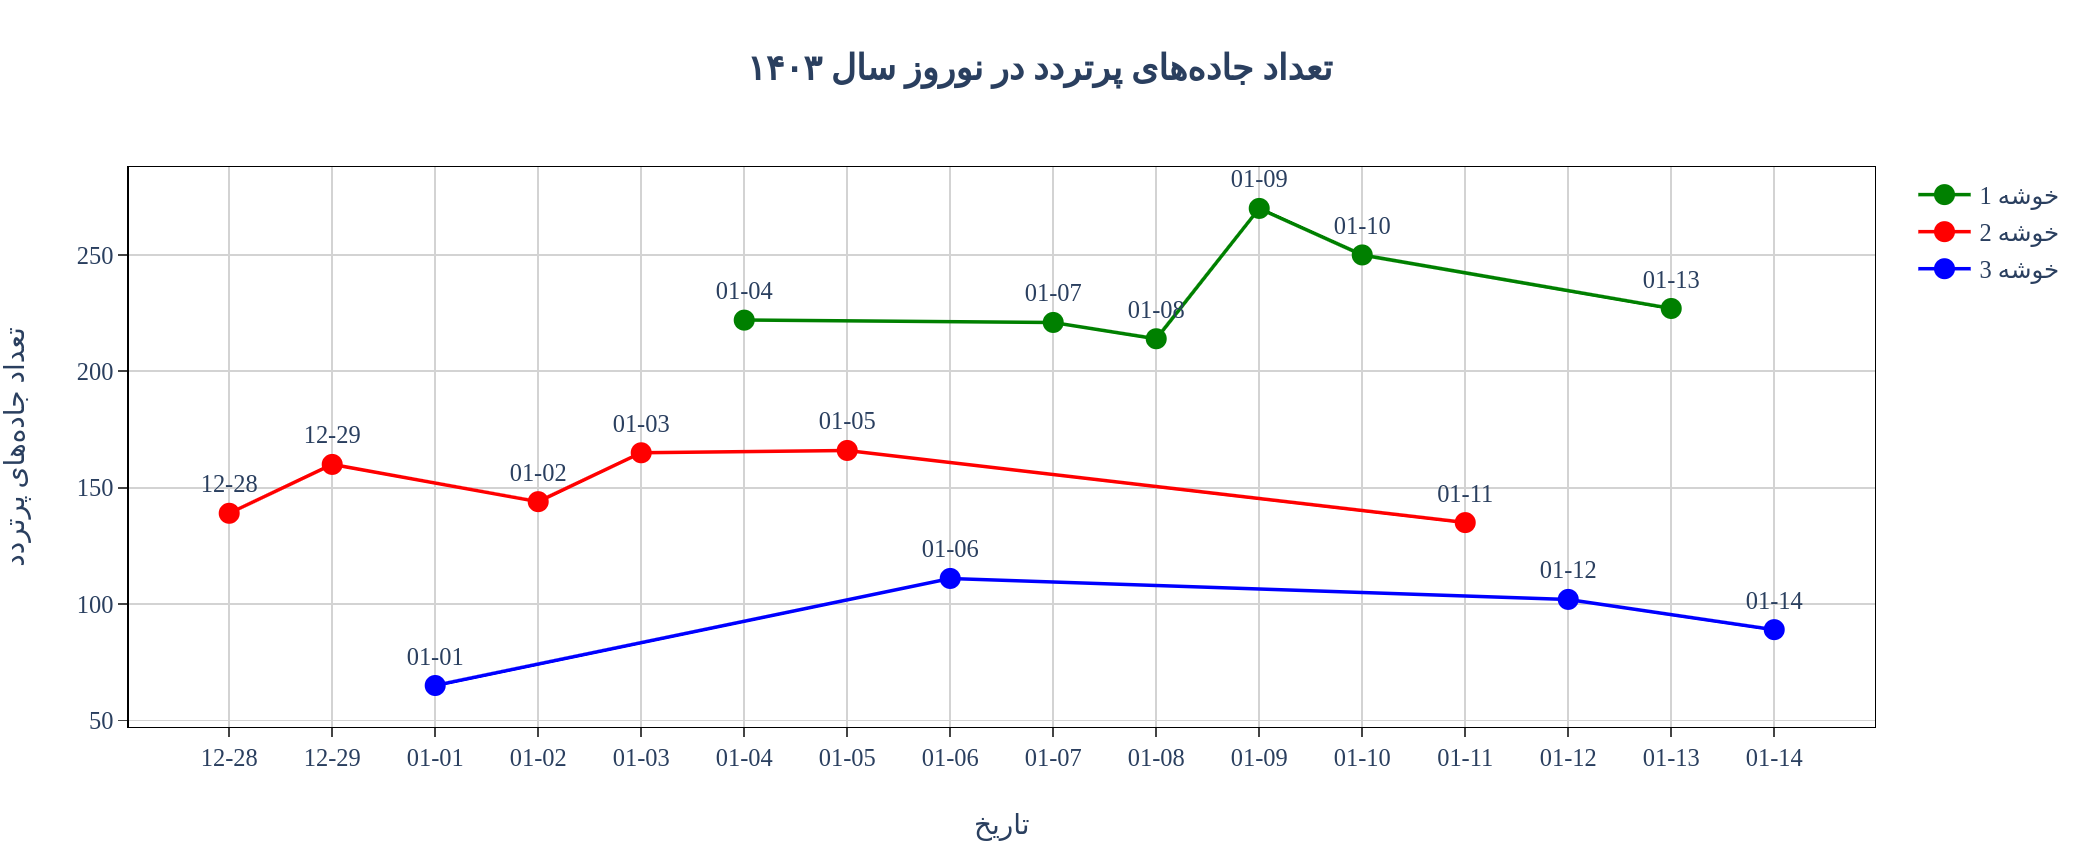
\includegraphics[width=0.8\textwidth]{peaks-pics/cluster1403.png}
    \caption{نمودار تعداد سواری‌ها در آزادراه شاهین شهر-اصفهان در نوروز ۱۴۰۲ و ۱۴۰۳}
\end{figure}

با بررسی الگوهای سفر در دو سال اخیر، می‌توان به یک تصویر کلی از رفتار ترافیکی نوروز دست یافت که در بسیاری از مسیرها تکرار می‌شود. در این الگو، روزهای ۲۹ اسفند، ۴ فروردین، ۹ فروردین، ۱۰ فروردین و ۱۳ فروردین پرترددترین ایام تعطیلات به شمار می‌آیند. این روزها نمایانگر دو موج اصلی سفر هستند: موج نخست در روزهای منتهی به آغاز فروردین، و موج دوم در واپسین روزهای تعطیلات. در مقابل، روز ۶ فروردین معمولاً با کاهش نسبی تردد همراه است، که می‌تواند نشان‌دهنده‌ی تثبیت سفرها و اقامت مسافران در مقصد باشد. این وقفه میانی، یک الگوی رایج در رفتار سفرهای نوروزی به‌شمار می‌رود.

\begin{figure}[htbp]
    \centering
    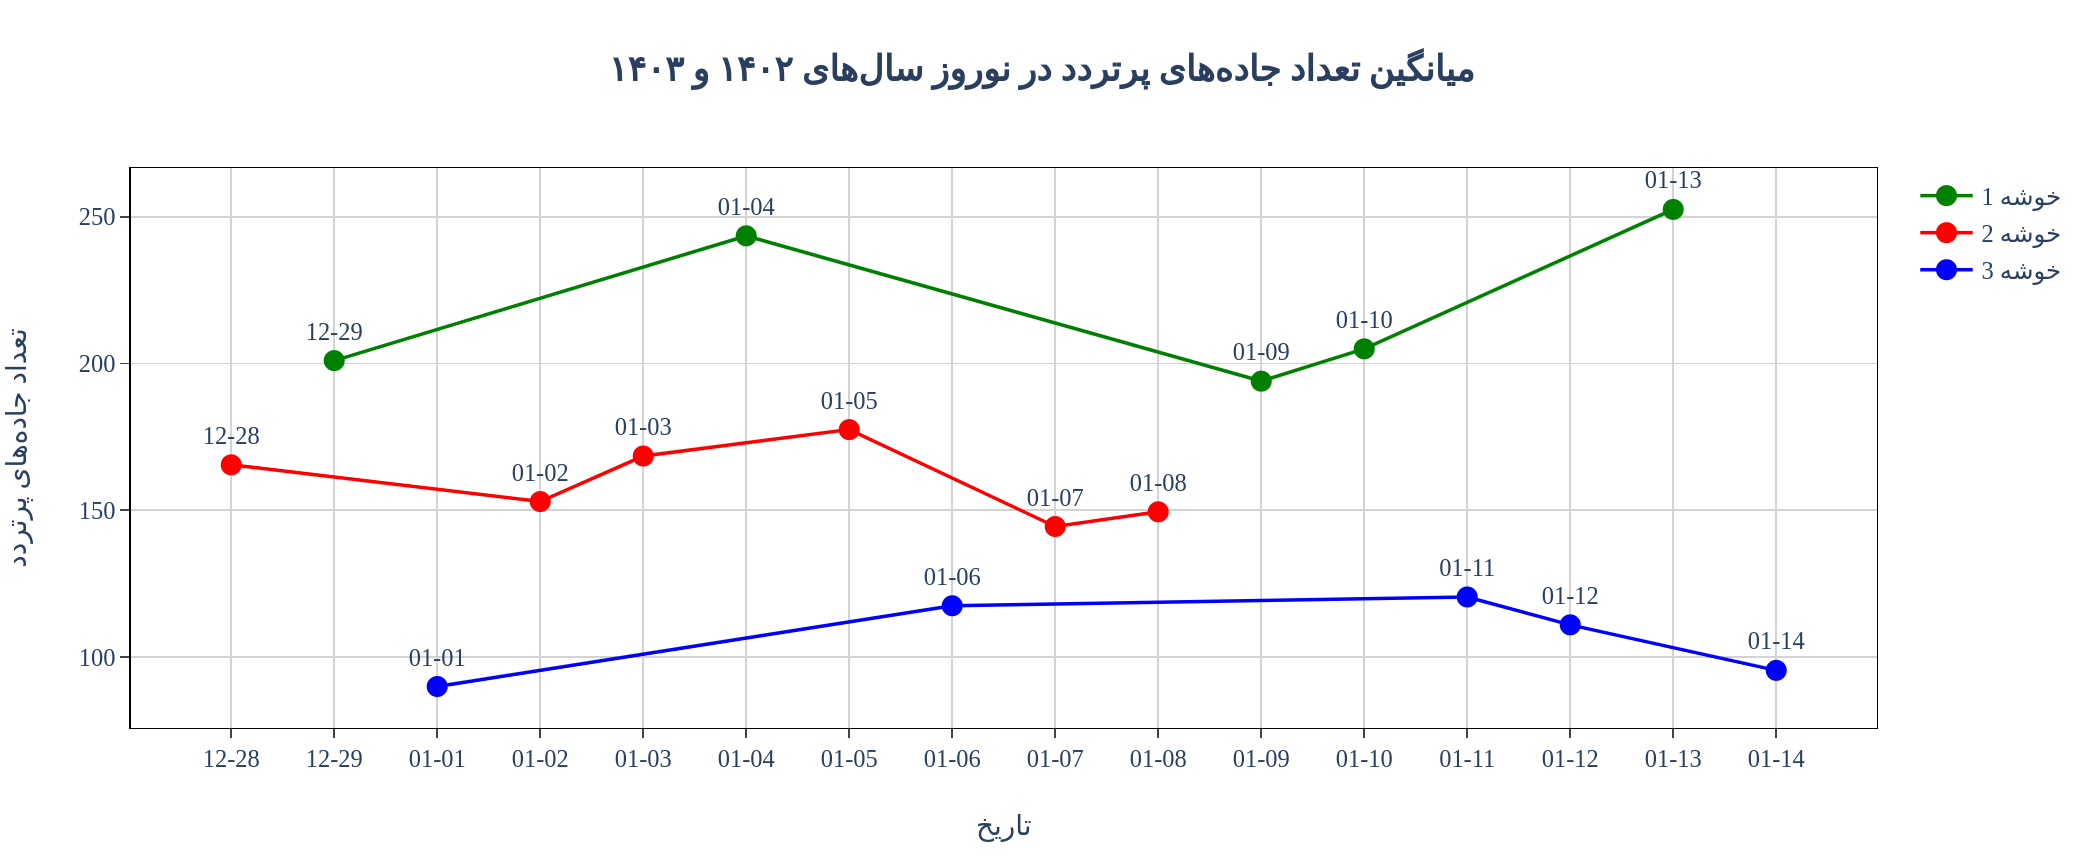
\includegraphics[width=0.8\textwidth]{peaks-pics/clustermean.png}
    \caption{نمودار تعداد سواری‌ها در آزادراه شاهین شهر-اصفهان در نوروز ۱۴۰۲ و ۱۴۰۳}
\end{figure}

درک دقیق این الگوهای زمانی، به برنامه‌ریزان حمل‌ونقل و مسئولان ترافیکی کشور کمک می‌کند تا بتوانند اقدامات مدیریتی بهتری در زمان‌های پیک ترافیکی اجرا کرده و از بروز ترافیک در مسیرهای پرتردد جلوگیری کنند. از سوی دیگر، آگاهی عمومی نسبت به این بازه‌های زمانی می‌تواند به مسافران در انتخاب هوشمندانه‌تر زمان سفر کمک کند.

\section{توضیحات فنی!!!}

در این مطالعه، داده‌های خام ترددشمارهای جاده‌ای سراسر کشور برای سه بازه‌ی نوروزی سال‌های ۱۴۰۱، ۱۴۰۲ و ابتدای ۱۴۰۳ مورد بررسی قرار گرفت. هدف از این تحلیل، شناسایی الگوهای غیرعادی تردد وسایل نقلیه و استخراج روزهای پرتردد در بازه‌ی زمانی ۱۰ اسفند تا ۲۰ فروردین هر سال بود. در گام نخست، برای کاهش اثر تفاوت‌های ساختاری بین جاده‌ها و فراهم آوردن امکان مقایسه‌پذیری، تعداد تردد وسایل نقلیه (در همه‌ی کلاس‌های پنج‌گانه) در هر روز و برای هر جاده، نسبت به مقدار متناظر آن در سال ۱۴۰۱ نرمال‌سازی شد. به این ترتیب، تغییرات معنادار تردد هر جاده در سال‌های بعد، صرف‌نظر از تفاوت مطلق سطح تردد، قابل بررسی و مقایسه بود.

در ادامه، برای هر روز از بازه‌ی زمانی مورد نظر، تعداد جاده‌هایی که میزان تردد آن‌ها بیش از سه برابر انحراف معیار نرمال‌سازی‌شده از میانگین خود فاصله داشت، محاسبه شد. این جاده‌ها به عنوان جاده‌های «پرتردد» در آن روز در نظر گرفته شدند. تحلیل این شاخص در سطح ملی نشان داد که بازه‌ی زمانی میان ۲۸ اسفند تا ۱۳ فروردین، با افزایش معنادار تعداد جاده‌های پرتردد همراه بوده است؛ که می‌توان آن را به‌عنوان پیک سفرهای نوروزی در نظر گرفت.

\begin{figure}[htbp]
    \centering
    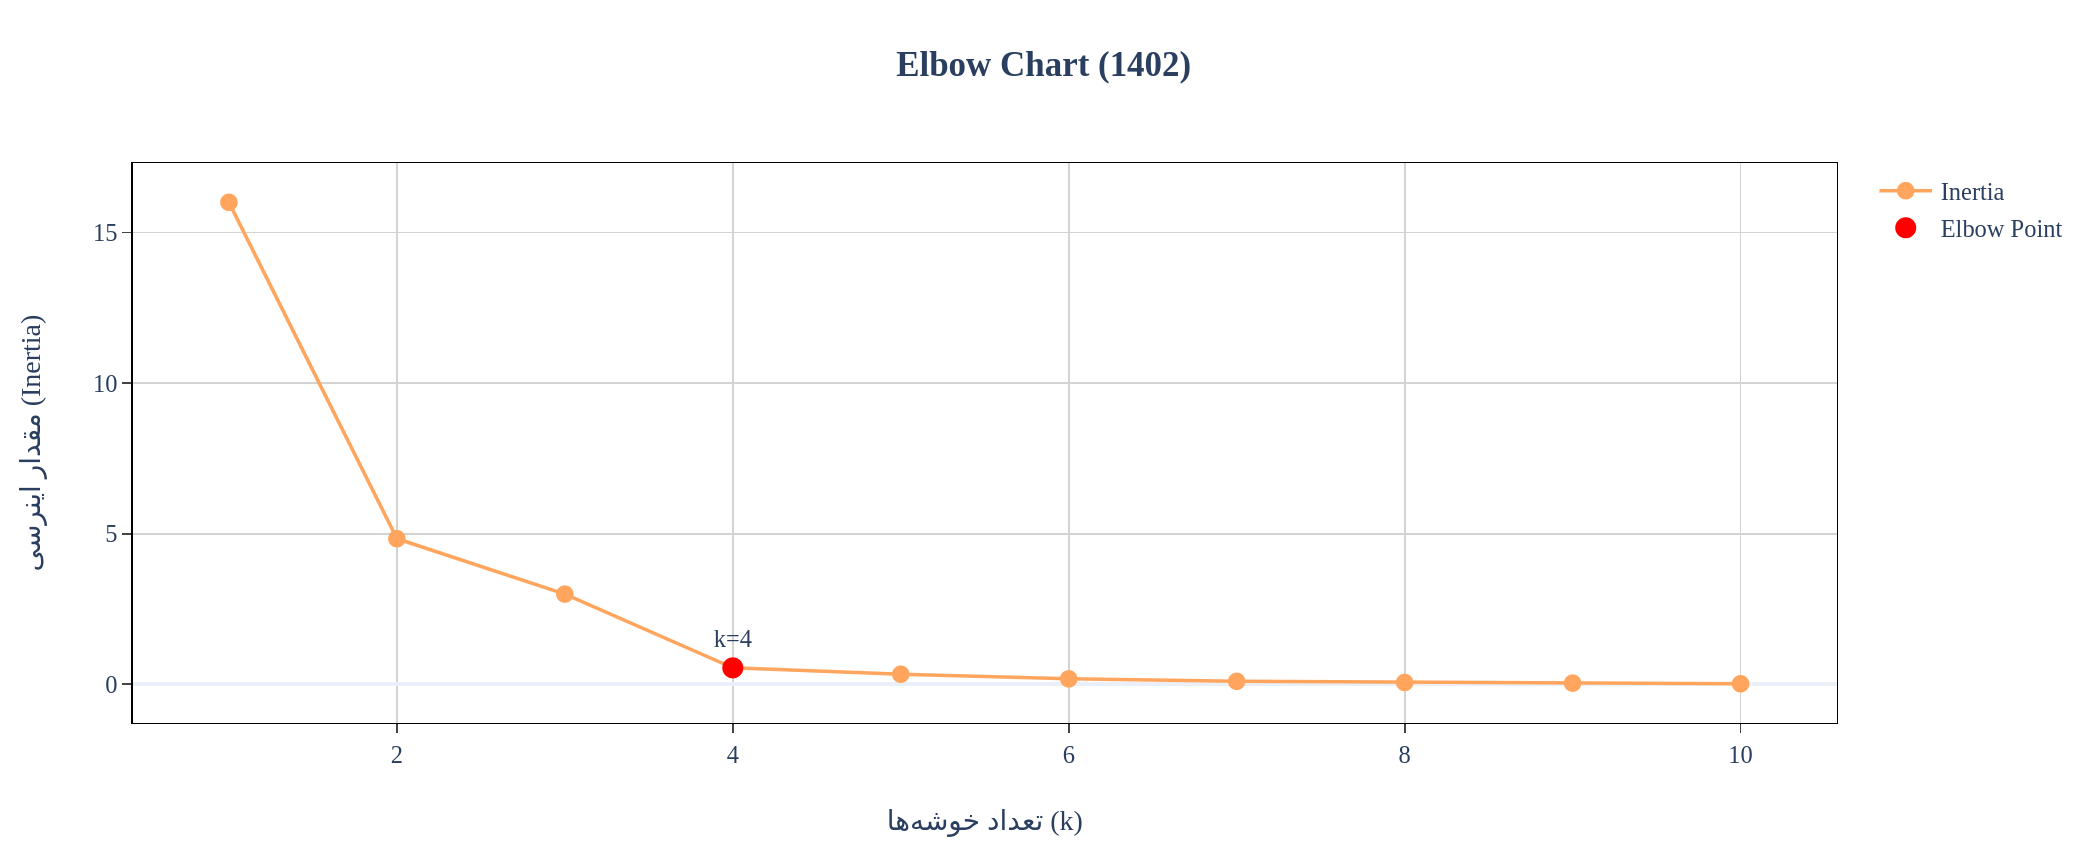
\includegraphics[width=0.8\textwidth]{peaks-pics/elbow1402.png}
    \caption{نمودار تعداد سواری‌ها در آزادراه شاهین شهر-اصفهان در نوروز ۱۴۰۲ و ۱۴۰۳}
\end{figure}

\begin{figure}[htbp]
    \centering
    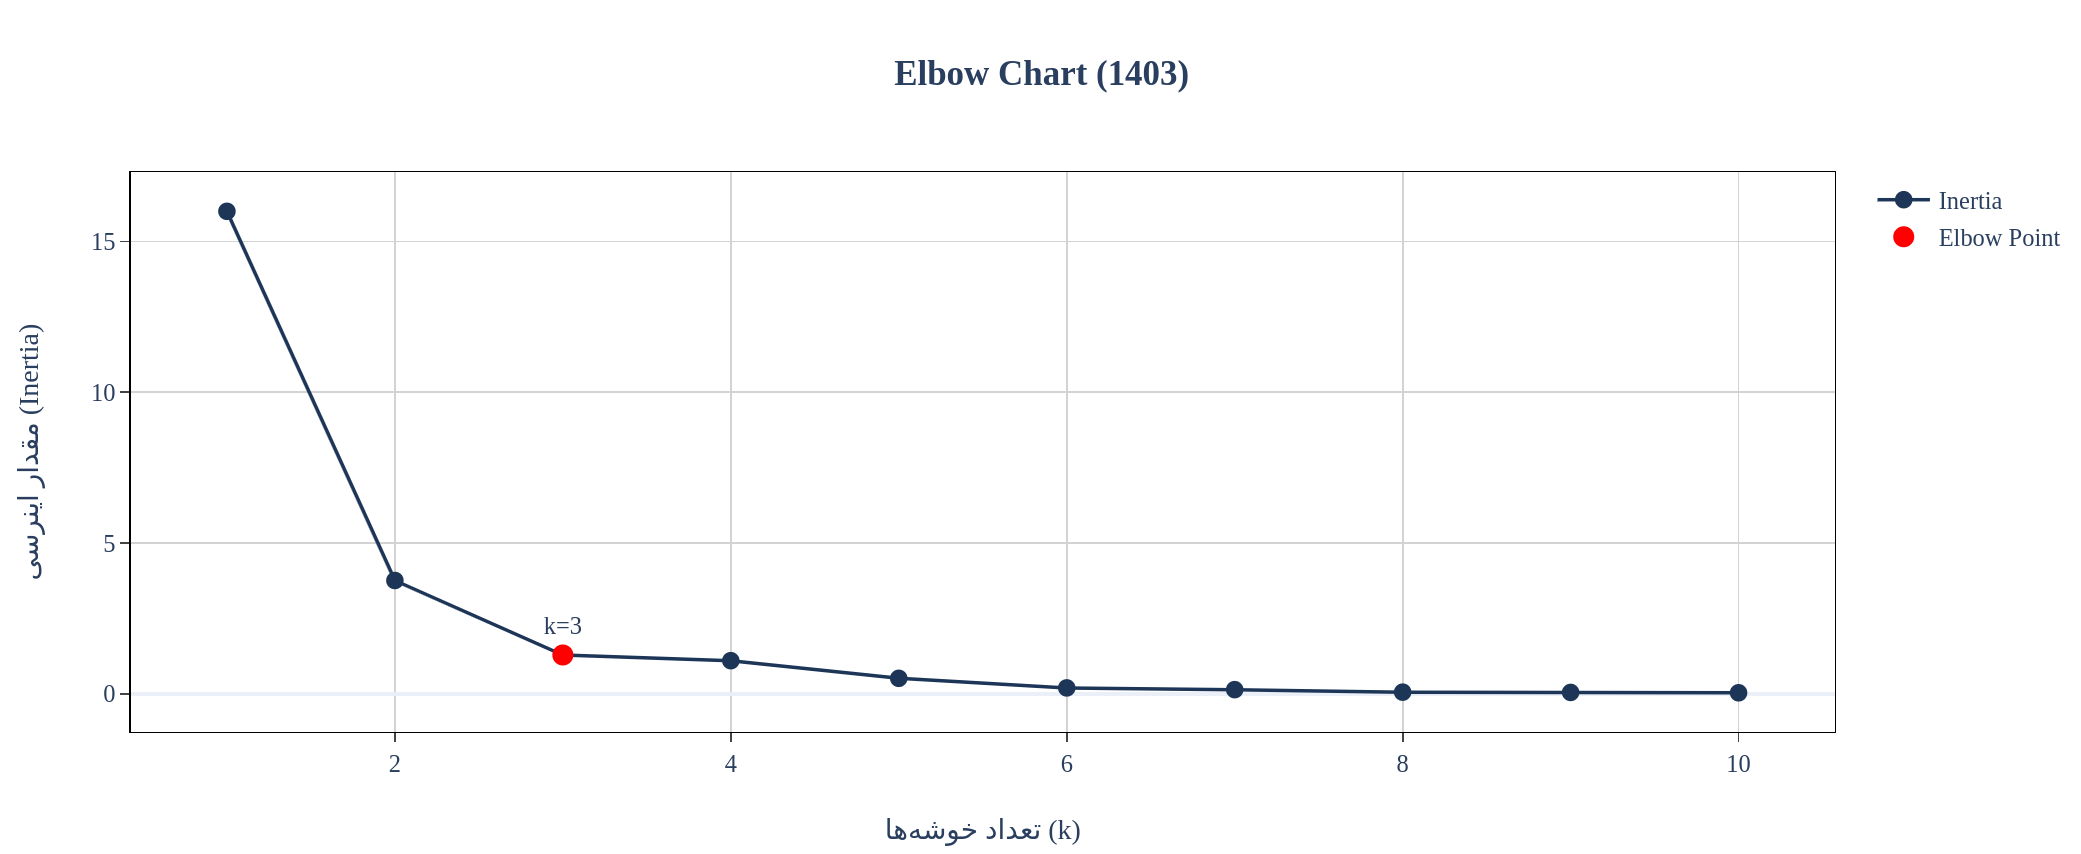
\includegraphics[width=0.8\textwidth]{peaks-pics/elbow1403.png}
    \caption{نمودار تعداد سواری‌ها در آزادراه شاهین شهر-اصفهان در نوروز ۱۴۰۲ و ۱۴۰۳}
\end{figure}

\begin{figure}[htbp]
    \centering
    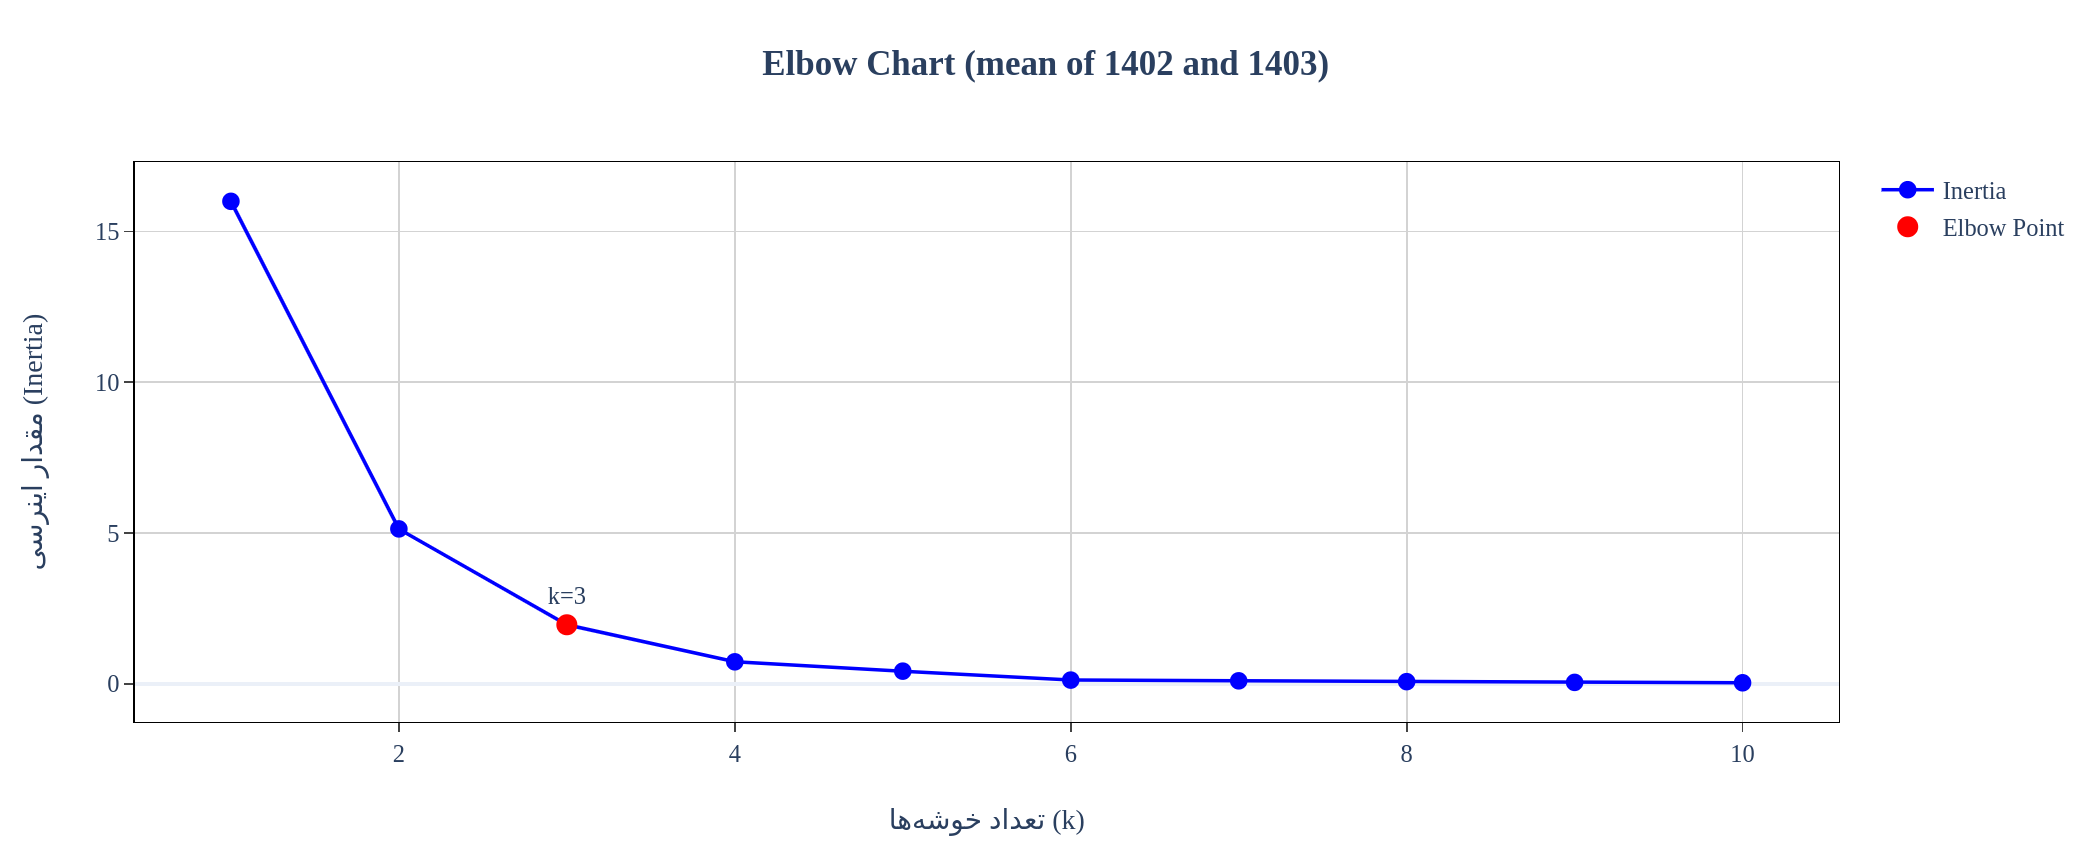
\includegraphics[width=0.8\textwidth]{peaks-pics/elbowmean.png}
    \caption{نمودار تعداد سواری‌ها در آزادراه شاهین شهر-اصفهان در نوروز ۱۴۰۲ و ۱۴۰۳}
\end{figure}

در مرحله‌ی بعد، به منظور درک بهتر الگوهای زمانی در دوره‌ی پیک سفر، داده‌های نرمال‌سازی‌شده‌ی این بازه وارد فرآیند خوشه‌بندی شدند. برای انتخاب تعداد مناسب خوشه‌ها، روش Elbow به کار گرفته شد و بر اساس نمودارهای حاصل، تعداد بهینه‌ی خوشه‌ها برای نوروز ۱۴۰۲ برابر با ۴ و برای نوروز ۱۴۰۳ برابر با ۳ تعیین شد. در نهایت، با در نظر گرفتن میانگین این مقادیر و نیز به منظور ساده‌سازی تفسیر، تعداد ۳ خوشه برای تحلیل نهایی انتخاب شد. نتایج این خوشه‌بندی در قالب سه نمودار جداگانه ارائه شده‌اند که توزیع روزهای پرتردد و الگوهای رفتاری آن‌ها را به تفصیل نشان می‌دهد.


\section{اعضای گروه}
\begin{itemize}
    \item پریساسادات موسوی - 401100239
    \item مهدی طاهری جانبازلو - 401100422
    \item محمد برکتین - 401100082
\end{itemize}

\end{document}